\documentclass[12pt, a4paper]{article}
\usepackage[utf8]{inputenc}
\usepackage{graphicx}
\usepackage{geometry}
\geometry{a4paper, margin=1in}
\usepackage{tabularx}
\usepackage{booktabs}
\usepackage{float}

\title{\textbf{Laporan Perhitungan Manual dan Implementasi \\ K-Means Clustering}}
\author{
\textbf{Nama Kelompok:} \\
1. Rizki Pratama Sunarko(240411100181) \\
2. Ainur Suharyanto (240411100154) \\
3. Wahyu Ari Ananda Fitrotul Huda (240411100148) \\
}
\date{\today}

\begin{document}

\maketitle

\vspace{-1.5em}
\begin{center}
    \textbf{Mata Kuliah:} Kecerdasan Komputasional \\
    \textbf{Dosen Pengampu:} Dr. ARIK KURNIAWATI S.Kom., M.T
\end{center}

\vspace{1.5em}

\section{Inisialisasi Centroid Awal}
Kita menggunakan 30 data yang diambil dari dataset \textbf{Mall\_Customers} dengan fitur yang digunakan adalah \textit{Annual Income} dan \textit{Spending Score}. Berdasarkan hasil metode Elbow, diasumsikan \textbf{$K$ optimal = 3}.

Kita memilih 3 data pertama sebagai centroid awal:
\begin{itemize}
    \item Centroid 1 (C1): $[15.00, 39.00]$
    \item Centroid 2 (C2): $[15.00, 81.00]$
    \item Centroid 3 (C3): $[16.00, 6.00]$
\end{itemize}

\section{Iterasi 1: Menghitung Jarak Data ke Tiap Centroid}
Kita menggunakan rumus \textit{Euclidean Distance}:
\[ d(A, B) = \sqrt{(x_a - x_b)^2 + (y_a - y_b)^2} \]

Berikut adalah jarak setiap data ke masing-masing centroid pada iterasi pertama:

\begin{table}[H]
    \centering
    \resizebox{\textwidth}{!}{
    \begin{tabular}{|c|c|c|c|c|c|c|c|}
        \hline
        \textbf{Data} & \textbf{Annual Income} & \textbf{Spending Score} & \textbf{Jarak ke C1} & \textbf{Jarak ke C2} & \textbf{Jarak ke C3} & \textbf{Jarak Terdekat} & \textbf{Kluster Baru} \\
        \hline
        Data-1  & 15.00 & 39.00 & 0.00  & 42.00 & 33.02 & 0.00  & C1 \\
        Data-2  & 15.00 & 81.00 & 42.00 & 0.00  & 75.01 & 0.00  & C2 \\
        Data-3  & 16.00 & 6.00  & 33.02 & 75.01 & 0.00  & 0.00  & C3 \\
        Data-4  & 16.00 & 77.00 & 38.01 & 4.12  & 71.00 & 4.12  & C2 \\
        Data-5  & 17.00 & 40.00 & 2.24  & 41.05 & 34.01 & 2.24  & C1 \\
        Data-6  & 17.00 & 76.00 & 37.05 & 5.39  & 70.01 & 5.39  & C2 \\
        Data-7  & 18.00 & 6.00  & 33.14 & 75.06 & 2.00  & 2.00  & C3 \\
        Data-8  & 18.00 & 94.00 & 55.08 & 13.34 & 88.02 & 13.34 & C2 \\
        Data-9  & 19.00 & 3.00  & 36.22 & 78.10 & 4.24  & 4.24  & C3 \\
        Data-10 & 19.00 & 72.00 & 33.24 & 9.85  & 66.07 & 9.85  & C2 \\
        Data-11 & 19.00 & 14.00 & 25.32 & 67.12 & 8.54  & 8.54  & C3 \\
        Data-12 & 19.00 & 99.00 & 60.13 & 18.44 & 93.05 & 18.44 & C2 \\
        Data-13 & 20.00 & 15.00 & 24.52 & 66.19 & 9.85  & 9.85  & C3 \\
        Data-14 & 20.00 & 77.00 & 38.33 & 6.40  & 71.11 & 6.40  & C2 \\
        Data-15 & 20.00 & 13.00 & 26.48 & 68.18 & 8.06  & 8.06  & C3 \\
        Data-16 & 20.00 & 79.00 & 40.31 & 5.39  & 73.11 & 5.39  & C2 \\
        Data-17 & 21.00 & 35.00 & 7.21  & 46.39 & 29.43 & 7.21  & C1 \\
        Data-18 & 21.00 & 66.00 & 27.66 & 16.16 & 60.21 & 16.16 & C2 \\
        Data-19 & 23.00 & 29.00 & 12.81 & 52.61 & 24.04 & 12.81 & C1 \\
        Data-20 & 23.00 & 98.00 & 59.54 & 18.79 & 92.27 & 18.79 & C2 \\
        Data-21 & 24.00 & 35.00 & 9.85  & 46.87 & 30.08 & 9.85  & C1 \\
        Data-22 & 24.00 & 73.00 & 35.17 & 12.04 & 67.48 & 12.04 & C2 \\
        Data-23 & 25.00 & 5.00  & 35.44 & 76.66 & 9.06  & 9.06  & C3 \\
        Data-24 & 25.00 & 73.00 & 35.44 & 12.81 & 67.60 & 12.81 & C2 \\
        Data-25 & 28.00 & 14.00 & 28.18 & 68.25 & 14.42 & 14.42 & C3 \\
        Data-26 & 28.00 & 82.00 & 44.92 & 13.04 & 76.94 & 13.04 & C2 \\
        Data-27 & 28.00 & 32.00 & 14.76 & 50.70 & 28.64 & 14.76 & C1 \\
        Data-28 & 28.00 & 61.00 & 25.55 & 23.85 & 56.29 & 23.85 & C2 \\
        Data-29 & 29.00 & 31.00 & 16.12 & 51.92 & 28.18 & 16.12 & C1 \\
        Data-30 & 29.00 & 87.00 & 50.00 & 15.23 & 82.04 & 15.23 & C2 \\
        \hline
    \end{tabular}
    }
    \caption{Tabel Perhitungan Jarak dan Pengelompokan Kluster Iterasi 1}
\end{table}

\section{Iterasi 1: Memperbarui Centroid}
Centroid baru dihitung dari rata-rata (mean) setiap fitur pada masing-masing kluster:
\begin{itemize}
    \item \textbf{Kluster C1} memiliki 7 data.
    \begin{itemize}
        \item C1 Baru = Mean dari 7 data = $[22.43, 34.43]$
    \end{itemize}
    \item \textbf{Kluster C2} memiliki 15 data.
    \begin{itemize}
        \item C2 Baru = Mean dari 15 data = $[21.47, 79.67]$
    \end{itemize}
    \item \textbf{Kluster C3} memiliki 8 data.
    \begin{itemize}
        \item C3 Baru = Mean dari 8 data = $[20.62, 9.50]$
    \end{itemize}
\end{itemize}

\textit{Catatan: Langkah perhitungan jarak dan perbaruan centroid diulang terus hingga hasil centroid tidak berubah (konvergen).}

\section{Visualisasi Hasil}
Berikut adalah visualisasi hasil penentuan nilai K optimal menggunakan \textit{Elbow Method} beserta perbandingan hasil *clustering* K-Means menggunakan perhitungan \textit{from scratch} dan menggunakan fungsi *library*.

\begin{figure}[H]
    \centering
    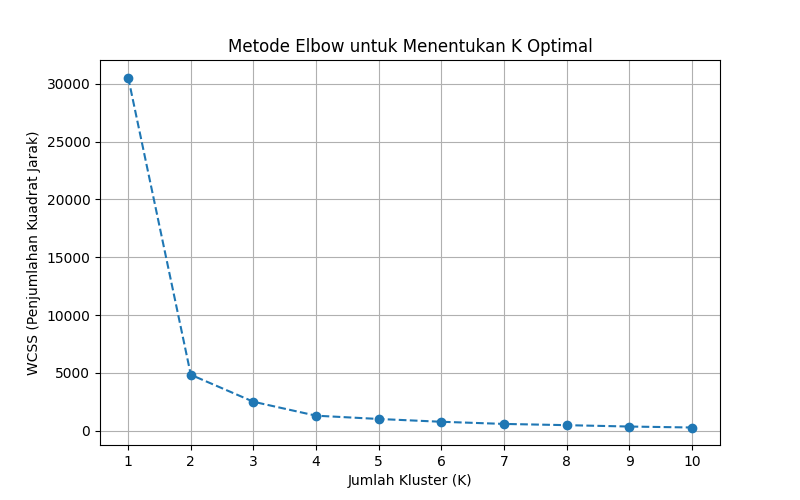
\includegraphics[width=0.8\textwidth]{image/elbow_method_library.png}
    \caption{Grafik Elbow Method (Menggunakan Library)}
\end{figure}

\begin{figure}[H]
    \centering
    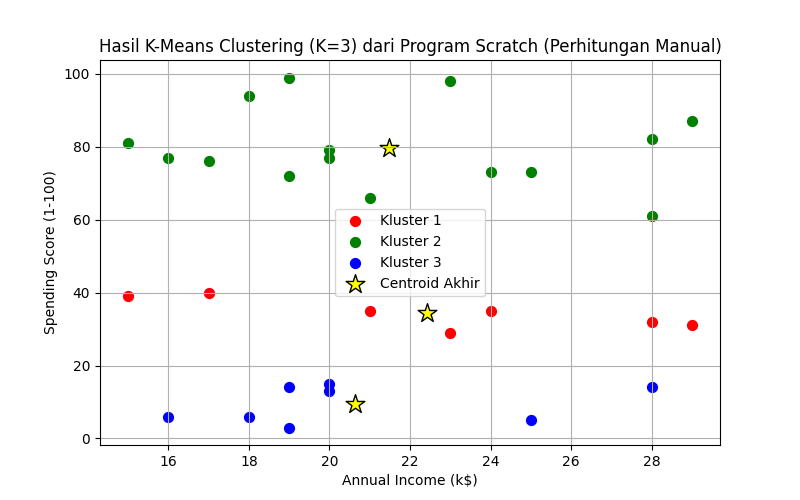
\includegraphics[width=0.8\textwidth]{image/hasil_clustering_scratch.png}
    \caption{Plot Visualisasi Hasil Clustering (Implementasi Algoritma Manual/Scratch)}
\end{figure}

\begin{figure}[H]
    \centering
    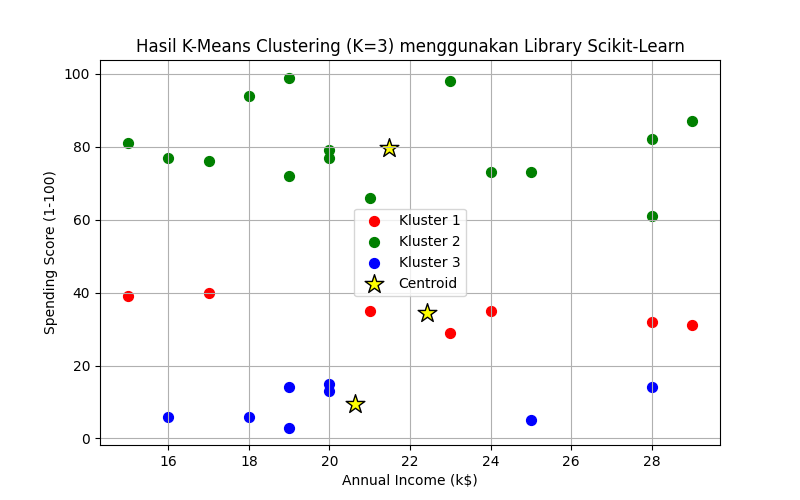
\includegraphics[width=0.8\textwidth]{image/hasil_clustering_library.png}
    \caption{Plot Visualisasi Hasil Clustering (Menggunakan Library Scikit-Learn)}
\end{figure}

\end{document}
